As Esferas Transdimensionais pousam serenamente, deixando entre cada uma o espaço necessário para os insetos desembarcarem. Ou melhor, para não se atrapalharem uns aos outros.

Depois mudam de cor, mesclam e avivam as cores, tornam-se azuis e estáticas.

As aberturas em cada bola começam a surgir, dão a volta a toda a superfície das esferas e desaparecem no lado oposto. Somem. E no seu lugar ficam os insetos, com o ar apatetado de quem viajou num outro mundo.

Então, o gafanhoto, que é meio deslocalizado, pergunta:
\bigbreak
— Estas bolas são fabulosas, podemos ficar com as ETs? Viajaríamos sempre juntos.
\bigbreak
\textbf{Eu sou Eu} sorri e diz:
\bigbreak
— Mas as ETs não existem. São Energia focada. Conseguiram viajar nelas com a anuência de Sírius. Serviram-nos no nosso passeio aqui neste planeta e, agora, dissolveram-se. São Energia livre.
\bigbreak
O vento que os sustentou na viagem resolve juntar-se à festa.

Sopra num campo de flores e uma chuva de polens de dentes-de-leão começa a cair no jardim. O sol, sempre atento e presente, pulsa-lhes a sua Luz e os pequenos grãos de pólen cintilam continuamente. Todo o jardim se arrepia.
\bigbreak
É a força da Primavera.
\bigbreak
Os insetos saltitam por todo lado e em alegria cantam:
\bigbreak
— Lá lá lá! Está a chover Pó das Estrelas. Lá lá lá. Está a chover Pó das Estrelas. Lá lá lá.
\bigbreak
O pequeno AnThaisiano compartilha da felicidade deles e da dádiva que os Elementos acabam de proporcionar. E sorrindo diz com ternura:
\bigbreak
— Neste planeta todos são Pó das Estrelas. O sopro do Criador, num ato repleto de Amor, disseminou Pólens e Sementes pelo Cosmos. Estes pólens e estas sementes são pequenas Partículas Divinas, que germinam incessantemente pelos mundos do Universo. Aos homens podemos chamar “Povo das Estrelas”, às plantas, “Plantas das Estrelas”, aos animais, “Animais das Estrelas”, às rochas, “Cristais das Estrelas” e a vocês meus pequeninos amigos... “Insetos das Estrelas”.

Ficam radiantes porque nunca tinham sido tão acarinhados. E agora sentem-se também viajantes das estrelas. \textbf{Eu sou Eu} continua:
\bigbreak
— Tudo o que existe, tudo o que vocês veem, foi e é criado com Amor. O Amor é a matriz e a força motriz da Existência. É invisível, mas está em toda a parte. É onipresente.
\bigbreak
— Lá lá lá. Nós somos o Amor. Lá lá lá. Nós somos o Amor. – os insetos começam outra vez a cantar.
\bigbreak
\textbf{Eu sou Eu} sente-se feliz naquele zunzum. E vai discorrendo:
\bigbreak
— Vocês são seres perfeitos. São pequeninas criaturas muito organizadas, simples, belas, trabalhadoras, colaborativas, construtivas e com muito mais predicados, mas o que é mesmo importante, é serem Unas e perceberem que a vida é uma brincadeira. Porque a grande e única responsabilidade real deste mundo é a de viver o Amor.
\bigbreak
— Os cristais, as flores, as montanhas, os mares e tudo o mais estão incluídos nesta palavra.
\bigbreak
— Os Elementos, que vos são tão próximos – a terra, a água, o ar e o fogo – misturam-se, sustentam e colorem a Vida. Os Elementos são Amor, porque o Amor é integração e inclusão. E também se encontram dentro de cada coração. Porque o coração é algo como... “cor em ação”. Com o coração damos cor e alegria à nossa vida.
\bigbreak
E continua a falar da magia dos Elementos:
\bigbreak
— Esta terra é o campo da matéria bruta onde o ar, como uma brisa suave ou um vento forte, carrega e dissemina as sementes e os pólens para nela germinarem. As nuvens, impulsionadas pelo vento, transportam por sua vez a água que depois cai em gotas de chuva e se infiltra na terra concebendo o húmus fertilizador. E o Sol, que é um fogo eterno, aquece toda essa mistura e faz nascer a Vida. O que é isto senão Amor?!
\bigbreak
— Gaia, incessantemente, cria a sua obra grandiosa com muita serenidade e na maior humildade, doando-a sem esperar retorno. Num verdadeiro Amor!
\bigbreak
— Amor, é o Sol que permanece no céu, dia após dia, irradiando ininterruptamente para todos sem distinção, e nunca diz que está cansado.
\bigbreak
— Da mesma maneira, dentro de cada coração, mesmo que ninguém se perceba, há um Sol colorido e eterno. O tal Amor em ação.
\bigbreak
— Amor, é cada floco de neve que tomba silenciosamente no chão, e que transporta em si um vitral de uma beleza imensurável, única e vibrante, e que ninguém vê.
\bigbreak
— Amor, é cada partícula de pólen que se agarra nas patinhas da abelha, viajando desprendida e sem olhar para trás, para num lugar longínquo fazer brotar a Vida.
\bigbreak
— O Amor envolve a noite, sempre que a mãe aconchega e beija o seu filho que dorme, e esse beijo é integrado no sonho da criança.
\bigbreak
— O Amor é...
\bigbreak
\textbf{Eu sou Eu} fala baixinho, mas as palavras vibram no ar e todos as recebem claramente.

E quem fica sem palavras são os insetos.

Mantêm-se no silêncio. Mas também não precisam delas, porque afinal, o Amor é apenas... o Amor.

E os ensinamentos verbais apenas servem àqueles que não compreendem o Silêncio.

\begin{figure}[h]
    \centering
    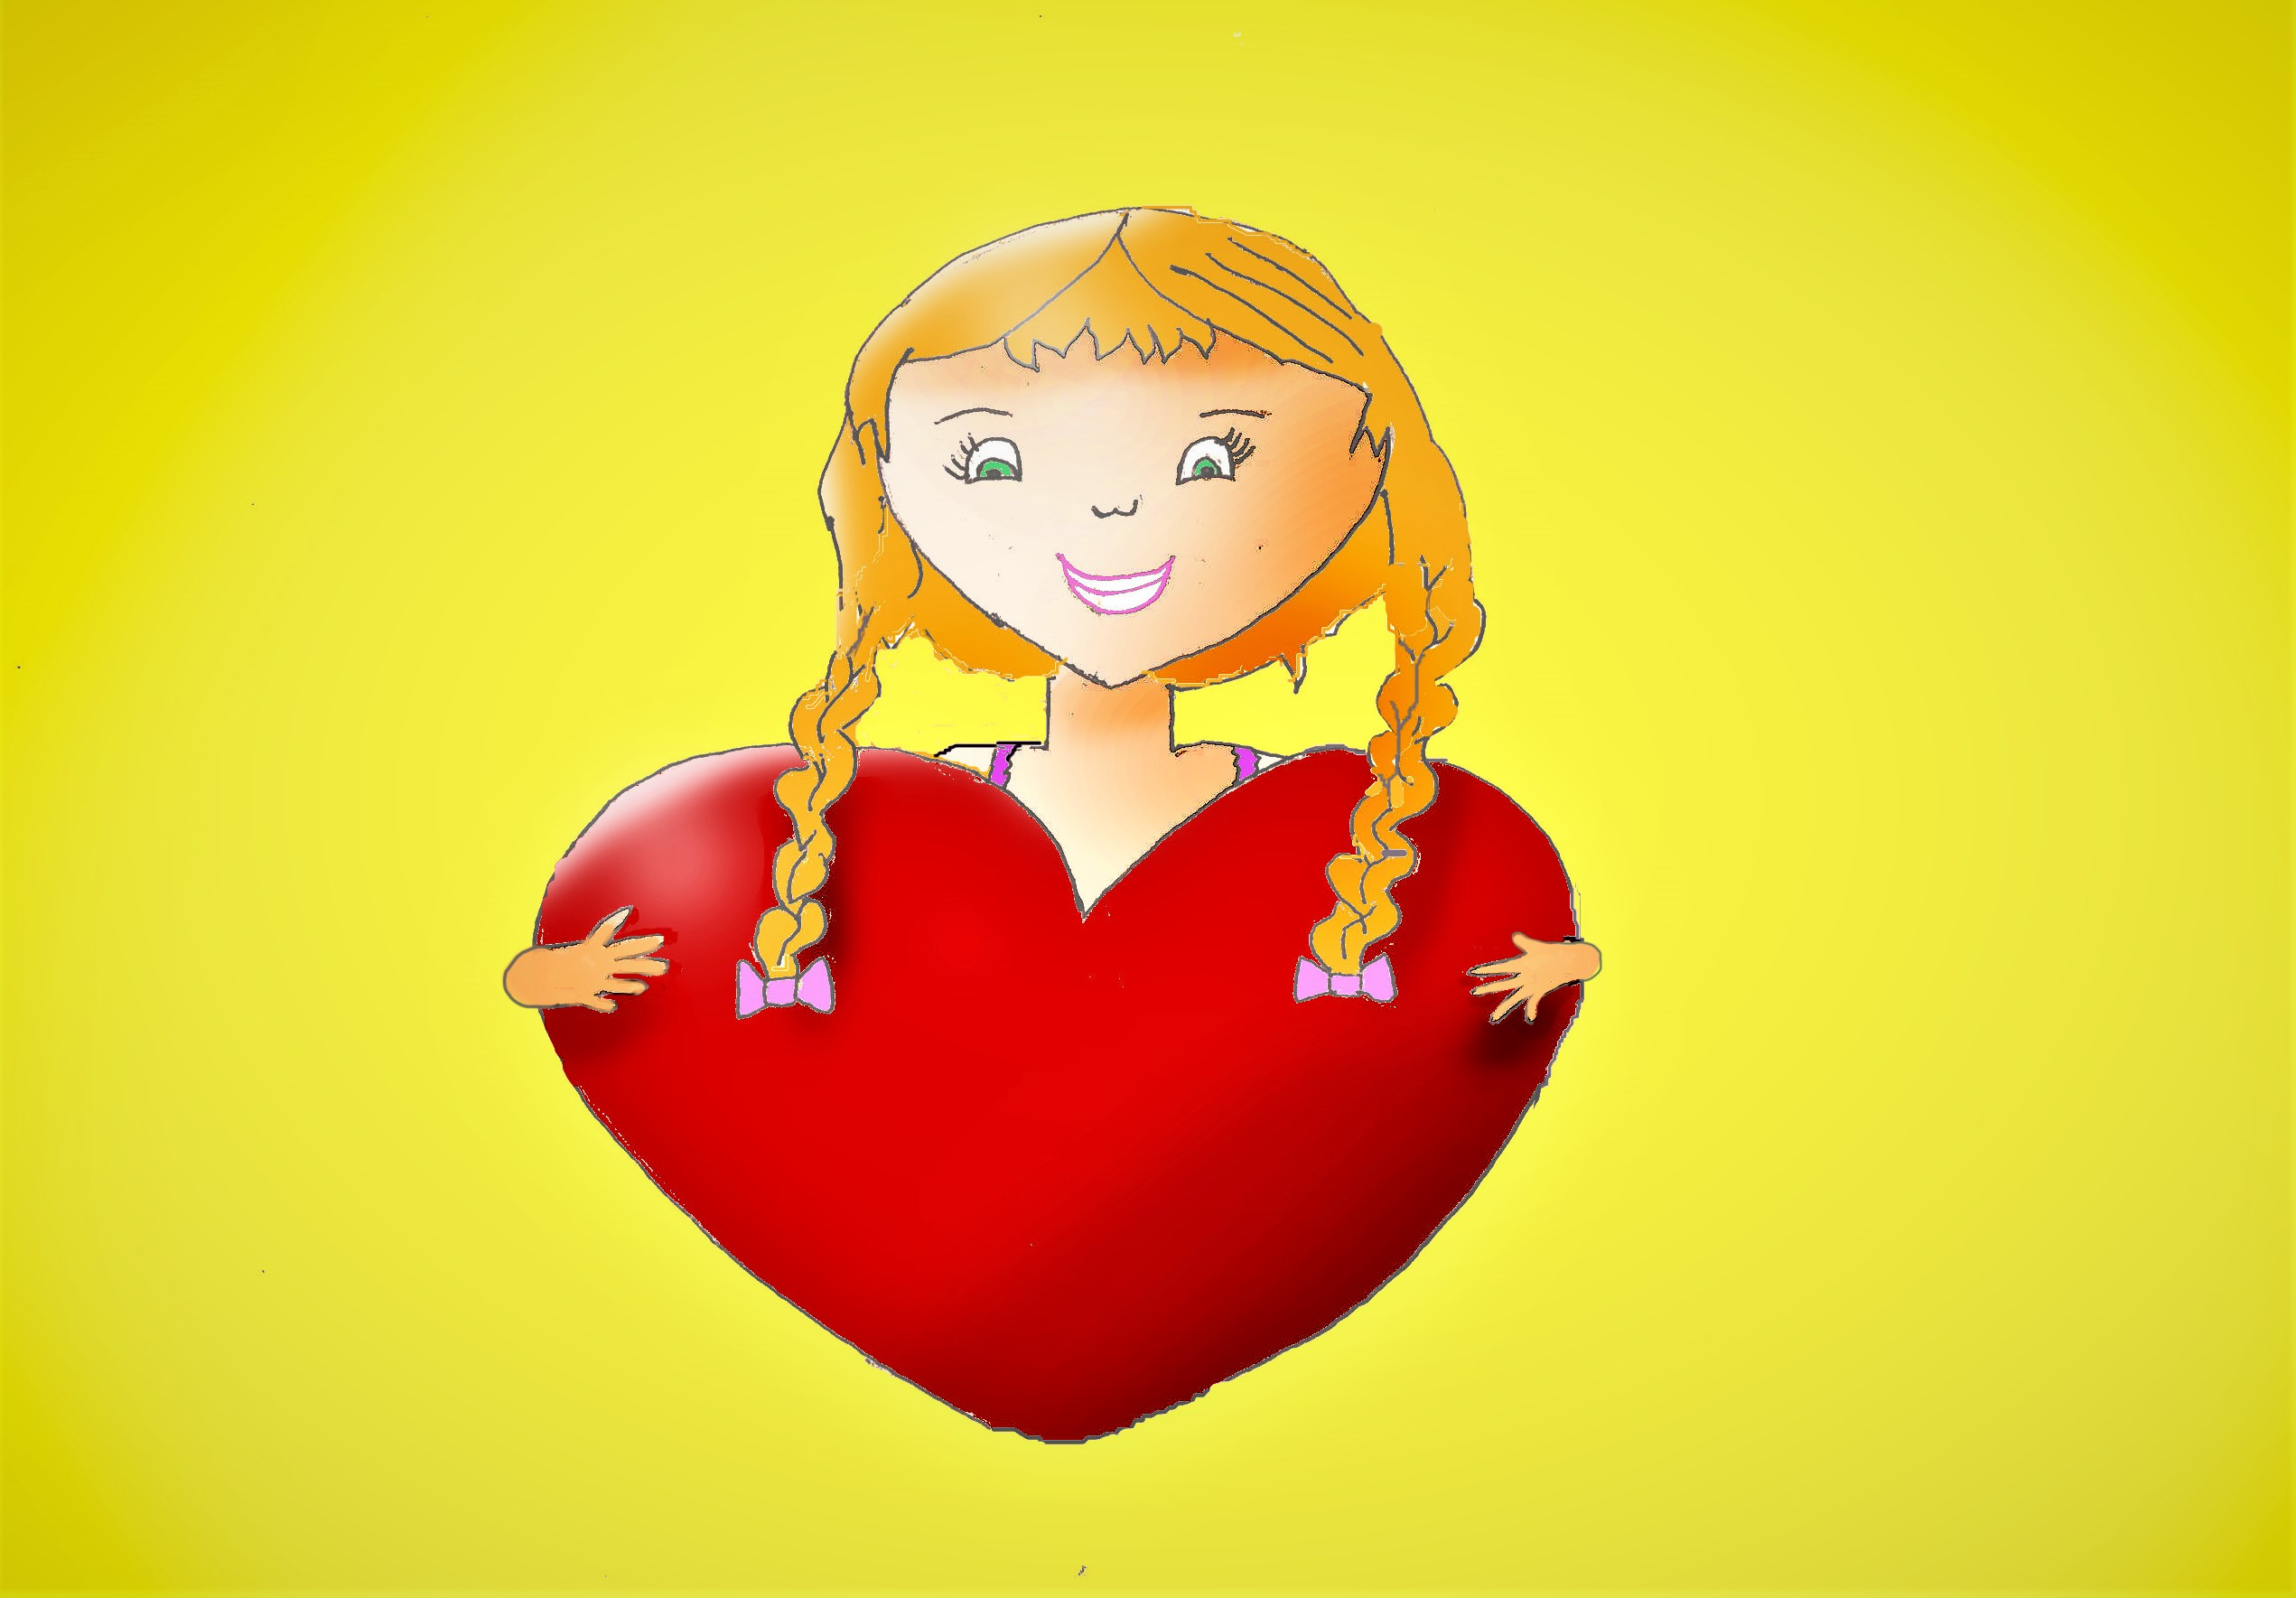
\includegraphics[width=0.85\textwidth]{coracao}
\end{figure}

\bigbreak
O AMOR é o TUDO,

O AMOR é o NADA.
